%%%%%%%%%%%%%%%%%%%%%%%%%%%%%%%%%%%%%%%%%%%%%%%%%%%%%%%%%%%%%%%%%%%%%%%%%%%%%%
%
% Appendix: Cluster Configuration
%
%%%%%%%%%%%%%%%%%%%%%%%%%%%%%%%%%%%%%%%%%%%%%%%%%%%%%%%%%%%%%%%%%%%%%%%%%%%%%%
\chapter{Cluster Configuration} \label{app:cluster-config}
The benchmark experiments for MySQL, MapReduce and Hive were executed on the
College of Engineering, Department of Computer Science, Onyx cluster at Boise
State University. The cluster has one master node (node00) and 32 compute nodes (node01-node32), 
which are connected with a private Broadcom Corporation NetXtreme BCM5754 Gigabit
Ethernet switch. Figure~\ref{fig:linux-cluster} shows the layout of the Onyx cluster lab.

\begin{figure}[h!]
 \centering
 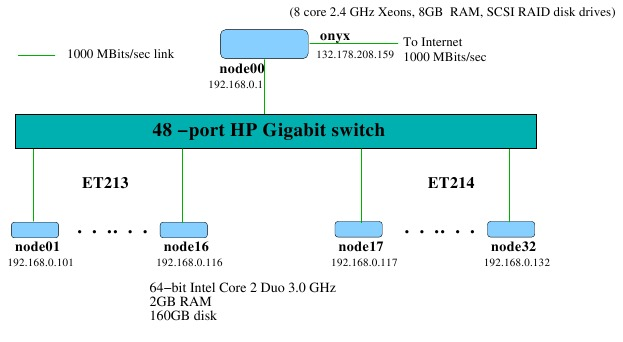
\includegraphics[bb=0 0 477 262]{../images/linux-cluster-lab.jpg}
 % linux-cluster-lab.jpg: 623x342 pixel, 94dpi, 16.84x9.24 cm, bb=0 0 477 262
 \caption{Boise State University, Department of Computer Science, Onyx Cluster Lab}
\label{fig:linux-cluster}
\end{figure}

Master node (node00) is an Intel(R) Xeon(R) E5530 @ 2.40GHz processor with
hyper-threading. It has a total of 8 processing threads (4 cores with 2 threads
per core) and 15K RPM SCSI drives with RAID-6.

Each compute node (node01-node32) is an Intel(R) Core(TM)2 Duo E8400 @ 3.00GHz
processor with 2 threads per node (2 cores with 1 thread per core). Each
compute node has a 7200 RPM SATA disk drive.